% Options for packages loaded elsewhere
\PassOptionsToPackage{unicode}{hyperref}
\PassOptionsToPackage{hyphens}{url}
%
\documentclass[
]{article}
\usepackage{amsmath,amssymb}
\usepackage{lmodern}
\usepackage{iftex}
\ifPDFTeX
  \usepackage[T1]{fontenc}
  \usepackage[utf8]{inputenc}
  \usepackage{textcomp} % provide euro and other symbols
\else % if luatex or xetex
  \usepackage{unicode-math}
  \defaultfontfeatures{Scale=MatchLowercase}
  \defaultfontfeatures[\rmfamily]{Ligatures=TeX, Scale=1}
\fi
% Use upquote if available, for straight quotes in verbatim environments
\IfFileExists{upquote.sty}{\usepackage{upquote}}{}
\IfFileExists{microtype.sty}{% use microtype if available
  \usepackage[]{microtype}
  \UseMicrotypeSet[protrusion]{basicmath} % disable protrusion for tt fonts
}{}
\makeatletter
\@ifundefined{KOMAClassName}{% if non-KOMA class
  \IfFileExists{parskip.sty}{%
    \usepackage{parskip}
  }{% else
    \setlength{\parindent}{0pt}
    \setlength{\parskip}{6pt plus 2pt minus 1pt}}
}{% if KOMA class
  \KOMAoptions{parskip=half}}
\makeatother
\usepackage{xcolor}
\usepackage{color}
\usepackage{fancyvrb}
\newcommand{\VerbBar}{|}
\newcommand{\VERB}{\Verb[commandchars=\\\{\}]}
\DefineVerbatimEnvironment{Highlighting}{Verbatim}{commandchars=\\\{\}}
% Add ',fontsize=\small' for more characters per line
\newenvironment{Shaded}{}{}
\newcommand{\AlertTok}[1]{\textcolor[rgb]{1.00,0.00,0.00}{\textbf{#1}}}
\newcommand{\AnnotationTok}[1]{\textcolor[rgb]{0.38,0.63,0.69}{\textbf{\textit{#1}}}}
\newcommand{\AttributeTok}[1]{\textcolor[rgb]{0.49,0.56,0.16}{#1}}
\newcommand{\BaseNTok}[1]{\textcolor[rgb]{0.25,0.63,0.44}{#1}}
\newcommand{\BuiltInTok}[1]{\textcolor[rgb]{0.00,0.50,0.00}{#1}}
\newcommand{\CharTok}[1]{\textcolor[rgb]{0.25,0.44,0.63}{#1}}
\newcommand{\CommentTok}[1]{\textcolor[rgb]{0.38,0.63,0.69}{\textit{#1}}}
\newcommand{\CommentVarTok}[1]{\textcolor[rgb]{0.38,0.63,0.69}{\textbf{\textit{#1}}}}
\newcommand{\ConstantTok}[1]{\textcolor[rgb]{0.53,0.00,0.00}{#1}}
\newcommand{\ControlFlowTok}[1]{\textcolor[rgb]{0.00,0.44,0.13}{\textbf{#1}}}
\newcommand{\DataTypeTok}[1]{\textcolor[rgb]{0.56,0.13,0.00}{#1}}
\newcommand{\DecValTok}[1]{\textcolor[rgb]{0.25,0.63,0.44}{#1}}
\newcommand{\DocumentationTok}[1]{\textcolor[rgb]{0.73,0.13,0.13}{\textit{#1}}}
\newcommand{\ErrorTok}[1]{\textcolor[rgb]{1.00,0.00,0.00}{\textbf{#1}}}
\newcommand{\ExtensionTok}[1]{#1}
\newcommand{\FloatTok}[1]{\textcolor[rgb]{0.25,0.63,0.44}{#1}}
\newcommand{\FunctionTok}[1]{\textcolor[rgb]{0.02,0.16,0.49}{#1}}
\newcommand{\ImportTok}[1]{\textcolor[rgb]{0.00,0.50,0.00}{\textbf{#1}}}
\newcommand{\InformationTok}[1]{\textcolor[rgb]{0.38,0.63,0.69}{\textbf{\textit{#1}}}}
\newcommand{\KeywordTok}[1]{\textcolor[rgb]{0.00,0.44,0.13}{\textbf{#1}}}
\newcommand{\NormalTok}[1]{#1}
\newcommand{\OperatorTok}[1]{\textcolor[rgb]{0.40,0.40,0.40}{#1}}
\newcommand{\OtherTok}[1]{\textcolor[rgb]{0.00,0.44,0.13}{#1}}
\newcommand{\PreprocessorTok}[1]{\textcolor[rgb]{0.74,0.48,0.00}{#1}}
\newcommand{\RegionMarkerTok}[1]{#1}
\newcommand{\SpecialCharTok}[1]{\textcolor[rgb]{0.25,0.44,0.63}{#1}}
\newcommand{\SpecialStringTok}[1]{\textcolor[rgb]{0.73,0.40,0.53}{#1}}
\newcommand{\StringTok}[1]{\textcolor[rgb]{0.25,0.44,0.63}{#1}}
\newcommand{\VariableTok}[1]{\textcolor[rgb]{0.10,0.09,0.49}{#1}}
\newcommand{\VerbatimStringTok}[1]{\textcolor[rgb]{0.25,0.44,0.63}{#1}}
\newcommand{\WarningTok}[1]{\textcolor[rgb]{0.38,0.63,0.69}{\textbf{\textit{#1}}}}
\usepackage{graphicx}
\makeatletter
\def\maxwidth{\ifdim\Gin@nat@width>\linewidth\linewidth\else\Gin@nat@width\fi}
\def\maxheight{\ifdim\Gin@nat@height>\textheight\textheight\else\Gin@nat@height\fi}
\makeatother
% Scale images if necessary, so that they will not overflow the page
% margins by default, and it is still possible to overwrite the defaults
% using explicit options in \includegraphics[width, height, ...]{}
\setkeys{Gin}{width=\maxwidth, height=\maxheight, keepaspectratio}
% Set default figure placement to htbp
\makeatletter
\def\fps@figure{htbp}
\makeatother
\setlength{\emergencystretch}{3em} % prevent overfull lines
\providecommand{\tightlist}{%
  \setlength{\itemsep}{0pt}\setlength{\parskip}{0pt}}
\setcounter{secnumdepth}{-\maxdimen} % remove section numbering
\ifLuaTeX
  \usepackage{selnolig}  % disable illegal ligatures
\fi
\IfFileExists{bookmark.sty}{\usepackage{bookmark}}{\usepackage{hyperref}}
\IfFileExists{xurl.sty}{\usepackage{xurl}}{} % add URL line breaks if available

\urlstyle{same} % disable monospaced font for URLs
\hypersetup{
  hidelinks,
  pdfcreator={KorigamiK LaTeX}}

\author{}
\date{}

\begin{document}

\section{\centering \LARGE{\underline{\href{https://github.com/korigamik/noted}{Noted}}}}

\begin{figure}
  \centering
  
\includegraphics[width=2.5cm]{./version-v0.1.0-green.png}
\end{figure}

A minimalist note-taking as well as sharing app.

\hypertarget{table-of-contents}{%
  \subsection{Table of Contents}\label{table-of-contents}}

\begin{itemize}
  \tightlist
  \item
        \protect\hyperlink{showcase}{Showcase}

        \begin{itemize}
          \tightlist
          \item
                \protect\hyperlink{home}{Home}
          \item
                \protect\hyperlink{sign-up}{Sign Up}
          \item
                \protect\hyperlink{log-in}{Log In}
          \item
                \protect\hyperlink{success}{Success}
          \item
                \protect\hyperlink{dashboard}{Dashboard}
          \item
                \protect\hyperlink{Logout}{Log Out}
          \item
                \protect\hyperlink{create}{Create}
          \item
                \protect\hyperlink{owned-notes}{Owned Notes}
          \item
                \protect\hyperlink{public-notes}{Public Notes}
          \item
                \protect\hyperlink{error}{Error}
        \end{itemize}
  \item
        \protect\hyperlink{highlights}{Highlights}
  \item
        \protect\hyperlink{development}{Development}
  \item
        \protect\hyperlink{known-issues}{Known Issues}
  \item
        \protect\hyperlink{license}{License}
\end{itemize}

\hypertarget{showcase}{%
  \pagebreak
  \subsection{Showcase}\label{showcase}
}

\hypertarget{home}{%
  \subsubsection{Home}\label{home}
  The minimalistic landing page of the app.
}

\begin{figure}[!h]
  \centering
  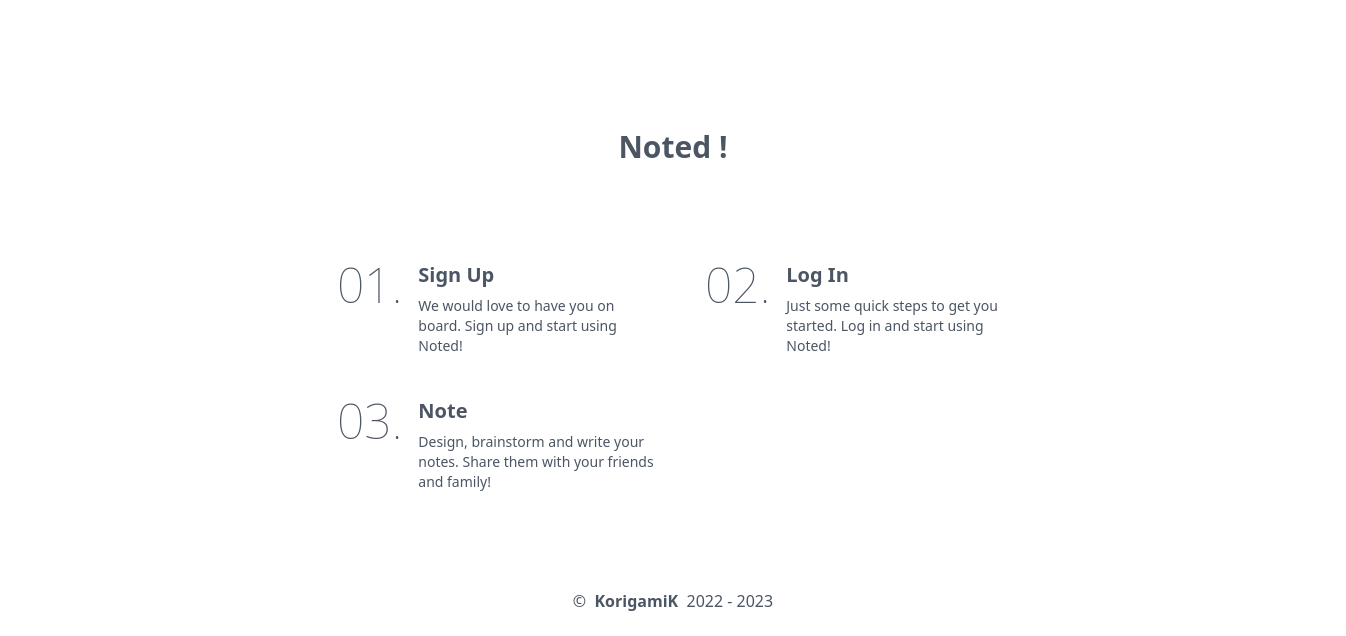
\includegraphics{../.github/images/home.png}
  \caption{Home}
\end{figure}

\hypertarget{sign-up}{
  \subsubsection{Sign Up}\label{sign-up}
  Hash the password and store the details on the database.
}

\begin{figure}[!h]
  \centering
  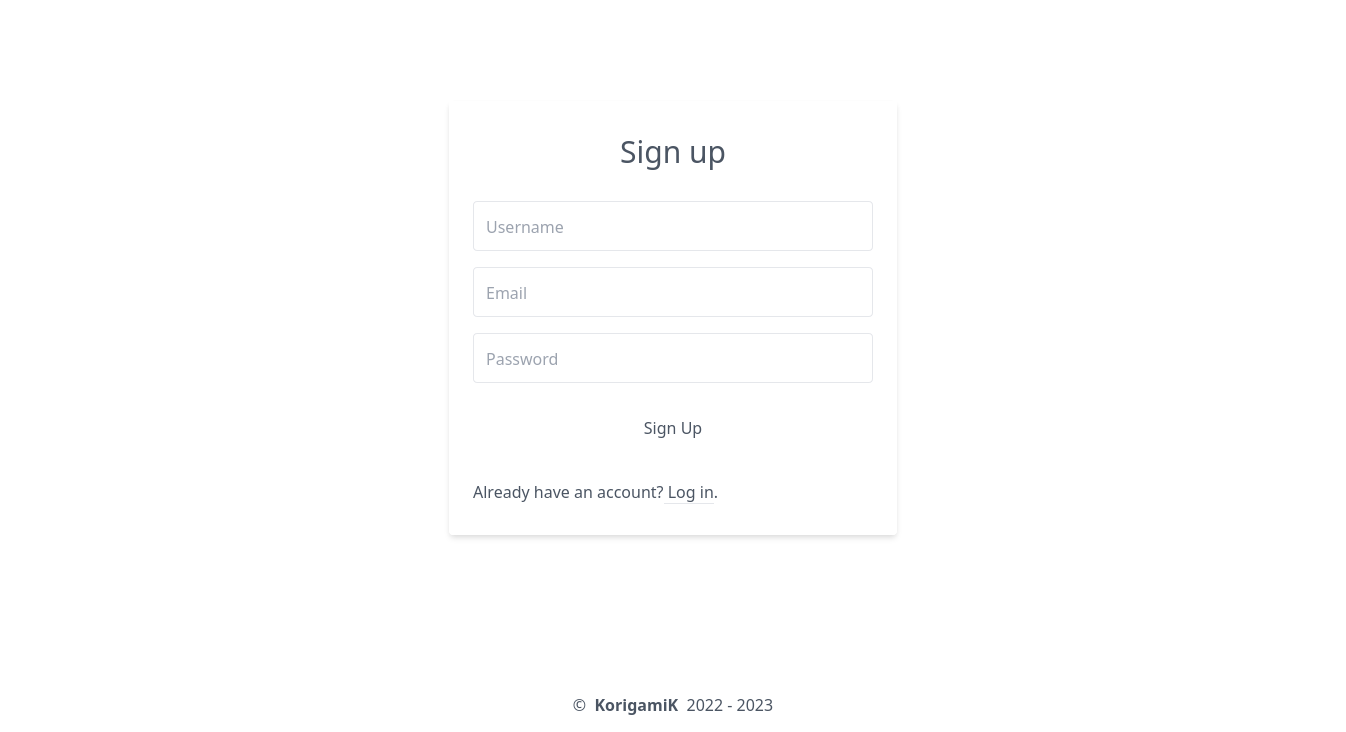
\includegraphics{../.github/images/signup.png}
  \caption{Home}
\end{figure}

\hypertarget{log-in}{
  \pagebreak
  \subsubsection{Log In}\label{log-in}
  A basic Email and Password authentication.
  This creates a persistent JWT cookie on the client.
}

\begin{figure}[!h]
  \centering
  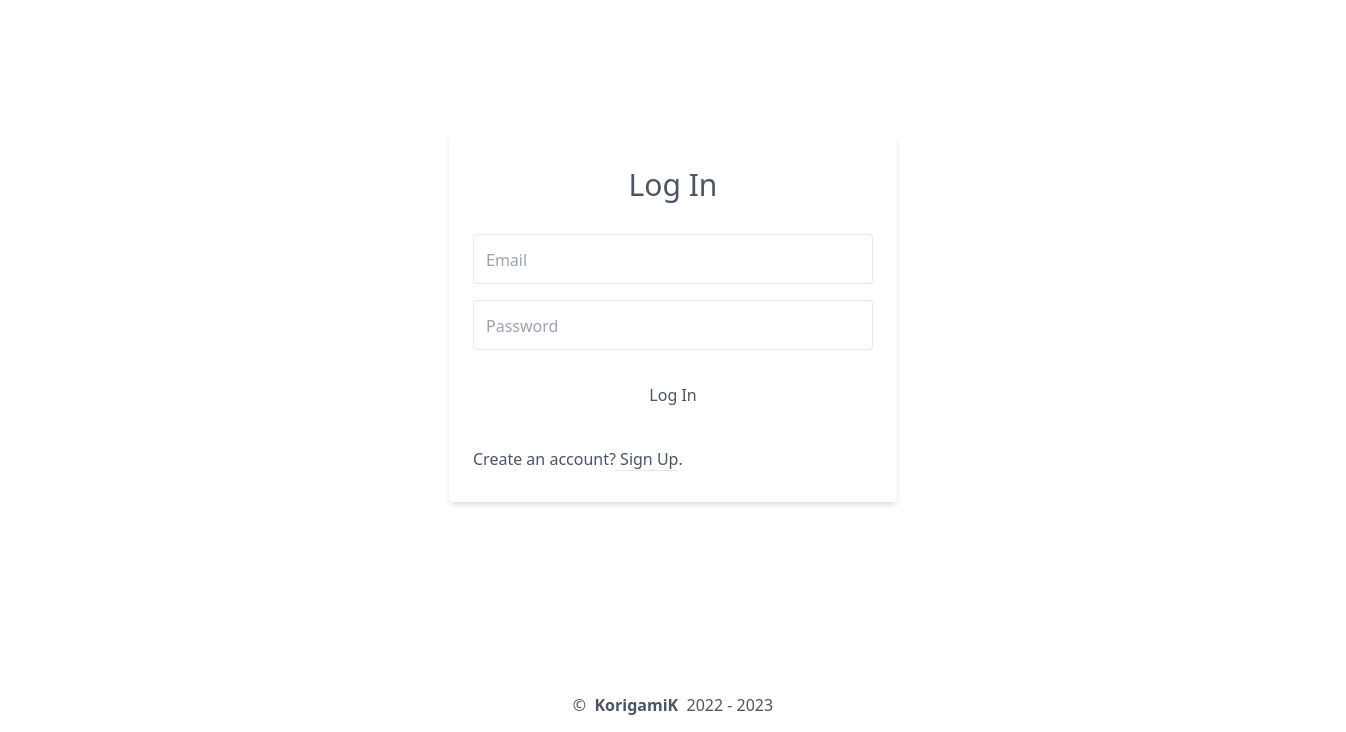
\includegraphics{../.github/images/login.png}
  \caption{Login}
\end{figure}

\hypertarget{success}{%
  \subsubsection{Success}\label{success}}

\begin{figure}[!h]
  \centering
  
\includegraphics{../.github/images/success.png}
  \caption{Success}
\end{figure}

\hypertarget{dashboard}{%
  \pagebreak
  \subsubsection{Dashboard}\label{dashboard}
  Create and view your repertoire of notes and share them with the world.
}

\begin{figure}[!h]
  \centering
  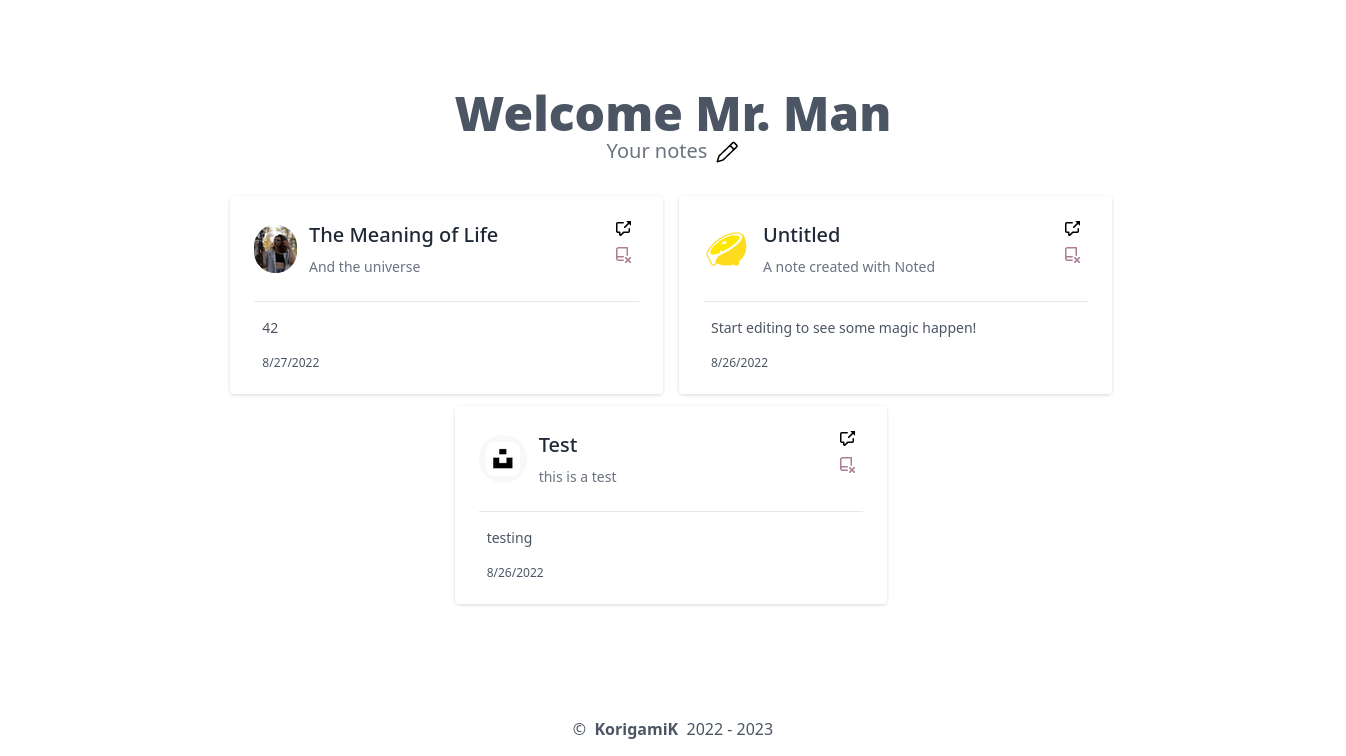
\includegraphics{../.github/images/dashboard.png}
  \caption{Dashboard}
\end{figure}

\hypertarget{create}{%
  \subsubsection{Create}\label{create}
  A new note will be created with the information provided when you save it.
}

\begin{figure}[!h]
  \centering
  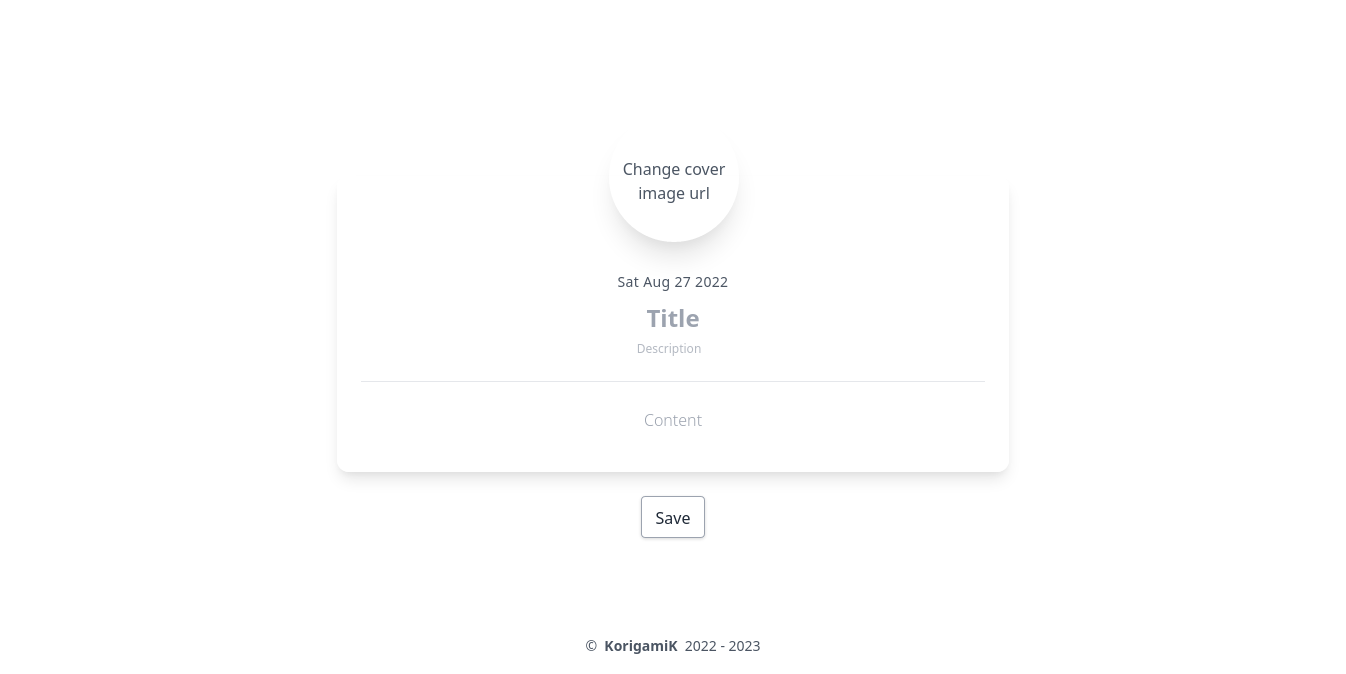
\includegraphics{../.github/images/create.png}
  \caption{Create}
\end{figure}

\hypertarget{owned-notes}{%
  \pagebreak
  \subsubsection{Owned Notes}\label{owned-notes}
  The Edit button will allow you to edit the note.
}

\begin{figure}[!h]
  \centering
  
\includegraphics{../.github/images/ownedNote.png}
  \caption{Owned Notes}
\end{figure}

\hypertarget{public-notes}{%
  \subsubsection{Public Notes}\label{public-notes}
  These notes can be accessed by anyone with the unique url. For example,\\
  \href{https://noted.deno.dev/note/63090ba0f680d16e0785c984b2b4c0017b0b2b2}{\textit{The url for this note}}.
}

\begin{figure}[!h]
  \centering
  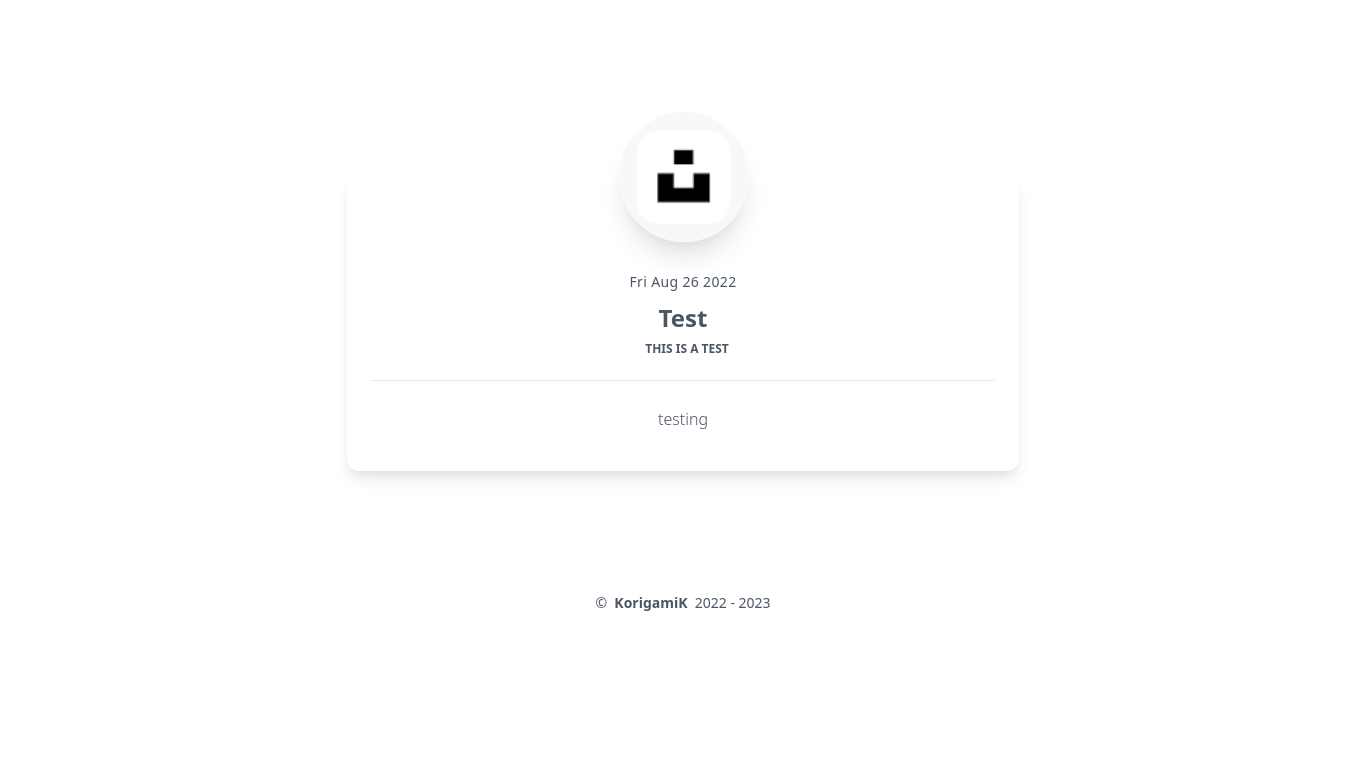
\includegraphics{../.github/images/publicNote.png}
  \caption{Public Notes}
\end{figure}

\hypertarget{error}{%
  \pagebreak
  \subsubsection{Error}\label{error}}

\begin{figure}[!h]
  \centering
  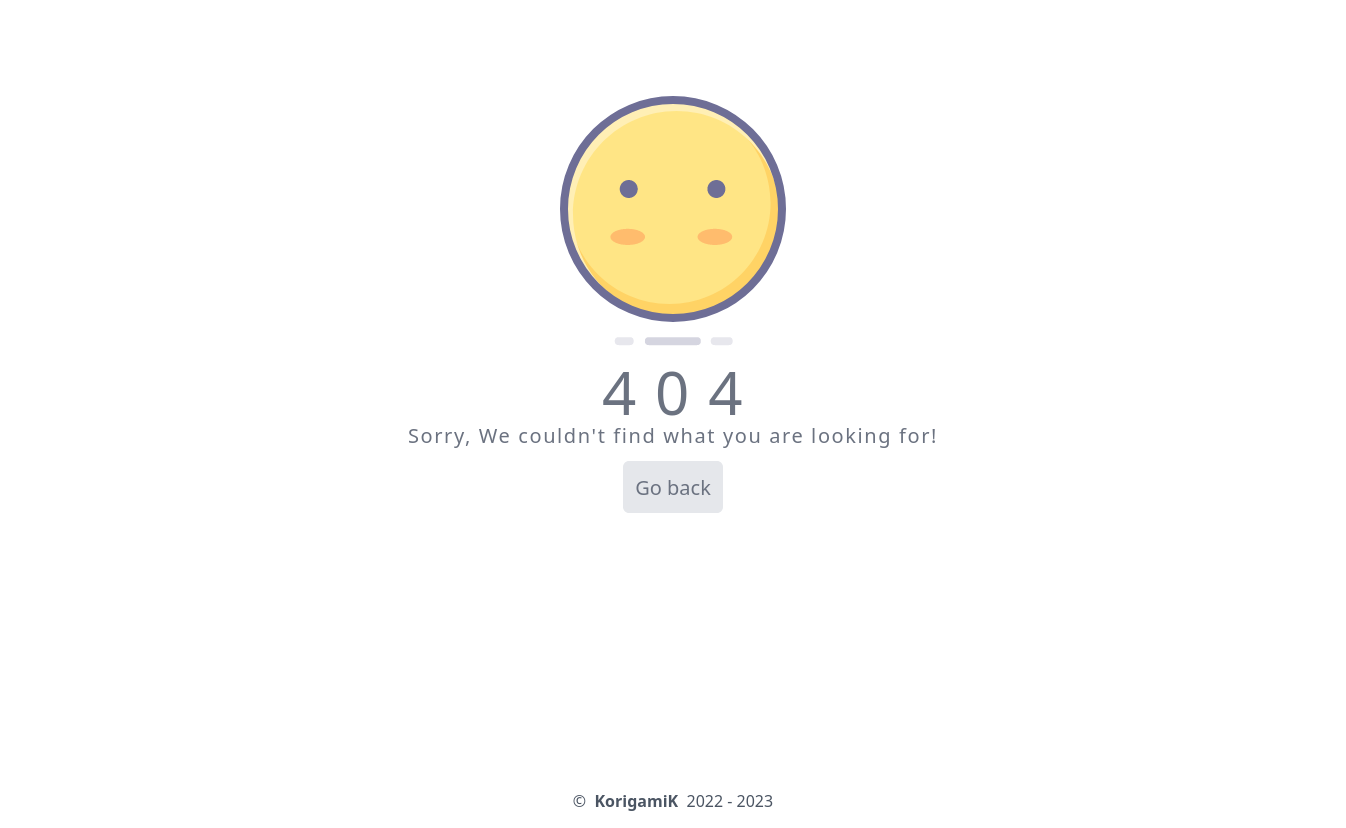
\includegraphics{../.github/images/error.png}
  \caption{Error}
\end{figure}

\hypertarget{Logout}{%
  \subsubsection{Logout}\label{Logout}
  The route to logout is \texttt{/logout}. which will log you out and redirect you to the home page.
}

\begin{figure}[!h]
  \centering
  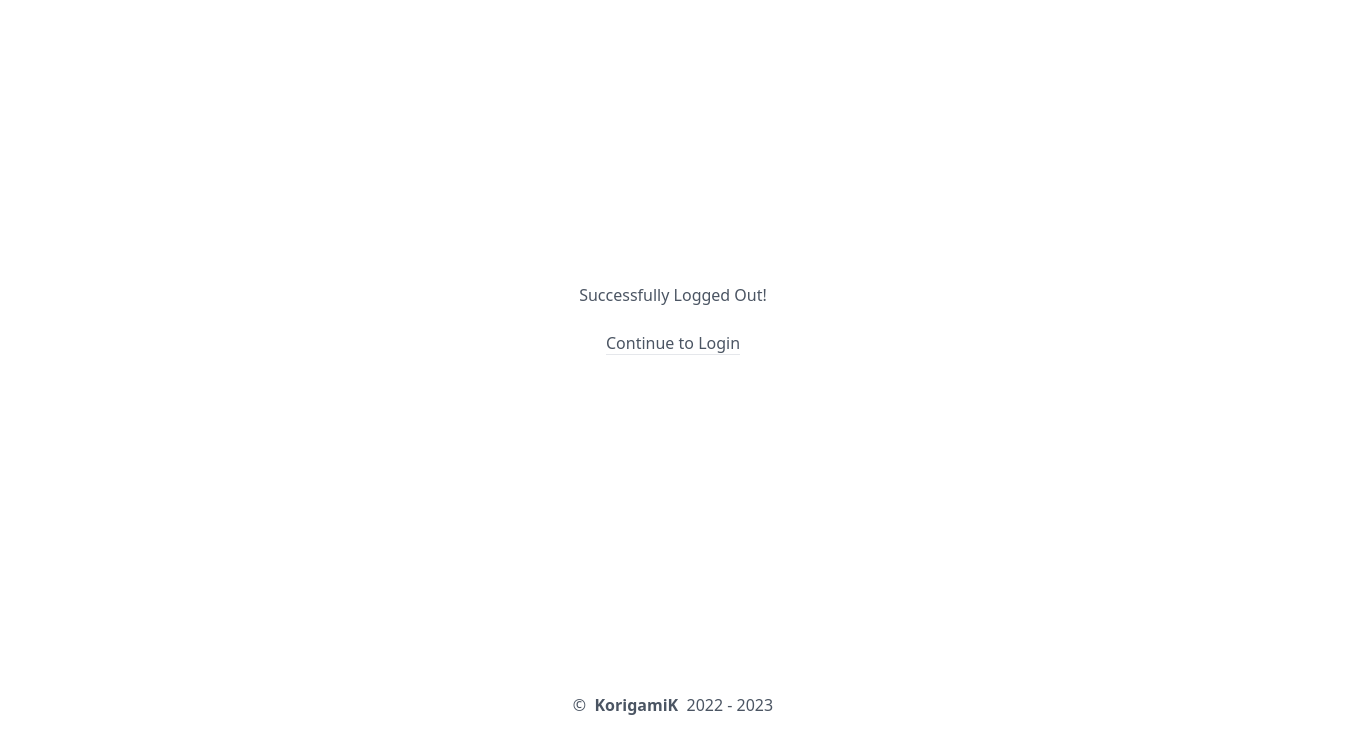
\includegraphics{../.github/images/logout.png}
  \caption{Logout}
\end{figure}

\hypertarget{highlights}{%
  \subsection{Highlights}\label{highlights}}

\begin{itemize}
  \tightlist
  \item
        Everything in TypeScript
  \item
        MongoDB with completely typed schema
  \item
        Persistent sessions using JSON Web Tokens (JWT)
  \item
        Free deployment using Deno deploy
  \item
        Public notes can be shared with anyone
  \item
        Using twind instead of tailwind
\end{itemize}

\hypertarget{development}{%
  \subsection{Development}\label{development}}

\begin{itemize}
  \tightlist
  \item
        Create a .env file in the root directory and set the following
        variables:

        \begin{itemize}
          \item
                \texttt{\_\_MONGO\_DB\_URI\_\_=} \linebreak
                \texttt{"mongodb+srv://\textless{}username\textgreater{}:\textless{}password\textgreater{}@\textless{}host-url\textgreater{}\linebreak/?authMechanism=SCRAM-SHA-1"}
          \item
                \texttt{\_\_DEVELOPMENT\_\_}= \texttt{True} If you want to persist
                logins across server restarts
        \end{itemize}
  \item
        Start the project:
        \begin{Shaded}
          \begin{Highlighting}[]
            \ExtensionTok{deno}\NormalTok{ task start}
          \end{Highlighting}
        \end{Shaded}
        This will watch the project directory and restart as necessary.
\end{itemize}

\hypertarget{known-issues}{%
  \subsection{Known Issues}\label{known-issues}}

\begin{itemize}
  \tightlist
  \item
        Web workers are not supported in Deno deploy. This means that async
        Bcrypt is not supported. This is a temporary issue and will be fixed
        in the future.

        \begin{itemize}
          \tightlist
          \item
                \href{https://github.com/JamesBroadberry/deno-bcrypt/issues/26}{Relevant
                  Issue}
        \end{itemize}
\end{itemize}

\hypertarget{license}{%
  \subsection{License}\label{license}}

\href{https://opensource.org/licenses/MIT}{
\includegraphics[width=2cm]{./License MIT.png}}

\href{https://fresh.deno.dev}{
\includegraphics[width=3cm]{./fresh-badge-dark.png}}

\AtEndDocument{\vfill \centering \pagenumbering{gobble} \copyright \href{https://github.com/korigamik/}{ KorigamiK}}

\end{document}
